\subsection{Анализ существующих решений}





\subsubsection{Оценка эффективности классических методов анализа фондового рынка}



\textbf{Фундаментальый анализ}

\par Методы фундаментального анализа вызывают разные оценки у специалистов \cite{classic-eff}. С одной стороны, фундаментальный анализ работает с реальными причинами движения цен –-- объективными факторами и причинноследственными закономерностями, известными в экономике и финансовой
науке. Обычно он проводится на нескольких уровнях –-- от макроэкономического до
уровня финансового состояния самого эмитента, благодаря чему формируется полноценное исследование объекта инвестирования и общей ситуации
принятия решений. Поэтому прогнозирование на его основе представляется
достаточно хорошо проработанным и экономически обоснованным.

\par С другой стороны применение фундаментального анализа содержит в себе и некоторые проблемы. Первая из них связана с гипотезой эффективного рынка. Основная предпосылка фундаментального анализа строится на том, что рыночная цена акции будет приближаться к своему «справедливому» значению ввиду действия гипотезы о рыночной эффективности. При этом забывается, что если бы данная гипотеза выполнялась, то наблюдаемая рыночная неэффективность с точки зрения базовой логики вообще не могла бы возникнуть.

\par В целом, методы фундаментального анализа являются достаточно
сложными, грамотное их использование доступно только профессиональным инвесторам и аналитикам, долгое время работающим на рынке. Важно также помнить о том, что возможным недостатком фундаментального анализа является его ориентация на долгосрочные вложения. 

\textbf{Технический анализ}

\par Методы технического анализа могут применяться для совершения
инвестиционных операций на современной бирже, однако эффективность данного метода находится под большим вопросом. \cite{classic-eff} Причиной сложившейся ситуации является ряд аргументов:

\begin{itemize}[leftmargin=1.6\parindent]
    \item[---] Технический анализ основан на использовании единственного
вида информации –-- цен прогнозируемого рыночного актива, поэтому с
его помощью невозможно оценить влияние иной информации;
	\item[---] Традиционные методы технического анализа являются чрезмерно упрощенными и не способны отражать сложные зависимости;
присутствующие в ценовой динамике рыночных активов;
    \item[---] В случае использования традиционных методов технического
анализа динамическая адаптация к происходящим на рынке изменениям отсутствует, что делает невозможным учет изменений, происходящих после настройки алгоритмов прогностической модели.
\end{itemize}

\textbf{Вывод об эффективности классических методов}

\par Основной вывод проведенного анализа, основанного на изучении
практики применения данных инструментов следующий – данные подходы имеют низкие прогностические возможности, явно недостаточные для обеспечения приемлемого уровня доходности, стабильной в
долгосрочной перспективе. Среди наиболее значительных недостатков можно выделить следующие:

\begin{itemize}[leftmargin=1.6\parindent]
	\item[---] Задействование чрезмерно малого количества факторов;
    \item[---] Фактически полное отсутствие аппарата преобразования проявления факторов
влияния в прогнозные значения динамики курсовых стоимостей акций;
    \item[---] Полная неизменность или крайне слабая изменяемость во времени зависимостей,
на основе которых осуществляется расчет прогнозных значений. 
\end{itemize}

\newpage

\subsubsection{Методы на основе теории детерминированного хаоса}

\par В работе \cite{chaos-based} на основе теории хаоса представлена непараметрическая модель для
прогнозирования будущего поведения валютных курсов. Теория хаоса предполагает, что
поведение финансовых рынков хаотично и обеспечивает основу для учета динамики нелинейных систем, которые могут выявлять скрытые шаблоны и тенденции в финансовых
данных, и которые, в свою очередь, не могут быть получены обычными статистическими
методами. Предложенная двухступенчатая модель сочетает в себе фазовое пространство,
реконструированное из одномерных хаотических временных рядов в комбинации с векторной регрессией.

\par Однако следует отметить, что в реальности биржевые рынки обладают свойством самоорганизации и памятью о предыдущих событиях, то есть не могут быть описаны в полной
мере теорией хаоса.

\par Данное направление является достаточно новым и говорить о его эффективности
пока, возможно, несколько преждевременно. На данный же момент, анализ
специализированной литературы показал \cite{chaos}, что практически все публикации, в которых
приводится описание прогностических инструментов на основе теории
детерминированного хаоса, относятся к периодической литературе, и многие из них
имеют явно рекламный характер. Ни в одном источнике не было обнаружено подробного
описания применения инструментов данного класса в условиях реального фондового
рынка, с указанием результатов, которые можно было бы считать достоверными и
устойчивыми во времени. Несмотря на то, что в публикациях, посвященных данному
направлению, иногда можно встретить описания положительных результатов применения
данного подхода в прогнозировании динамики курсовых стоимостей акций, они имеют
явно предвзятый характер.

\par Отзывы же практиков говорят прямо об обратном. Мнения непосредственных
инвесторов фондового рынка сводятся скорее к тому, что эффективность подобных
инструментов весьма сомнительна, и вряд ли можно утверждать, что она превышает
эффективность прогностических инструментов, созданных на основе традиционных
подходов. Поэтому и распространенность инструментов на основе теории
детерминированного хаоса среди инвесторов весьма мала.

\subsubsection{Инструменты на основе разработок в области ИИ}

\par Более длительную историю, по сравнению с теорией хаоса, имеет подход, основанный на применении для прогнозирования динамики курсовых стоимостей акций фондового рынка разработок в
области ИИ.
\par Искусственный интеллект --- раздел информатики, изучающий возможность
воспроизведения рассуждений и действий, аналогичных мышлению и действиям
человека, с помощью электронных вычислительных систем и иных искусственных
устройств. Главной задачей разработки систем искусственного интеллекта является
построение искусственной системы, например –-- компьютерной программы, обладающей
уровнем эффективности решения неформализованных задач, сравнимым с человеческим
или превосходящим его.
\par Исторически выделилось два основных подхода к построению систем ИИ:
логический и нейрокибернетический.
\par 1. Логический подход –-- математическое моделирование сознательной деятельности
человека, то есть моделирование высокоуровневых процессов мышления, основанных на
представлении и использовании знаний. Методология данного подхода - выявление и
применение в интеллектуальных системах различных логических и эмпирических
приемов (эвристик), которые человек использует для решения каких-либо задач. С
развитием в начале 80-х годов концепции экспертных систем это направление вылилось в
научно-технологическое направление информатики «инженерия знаний», занимающееся
созданием так называемых «систем, основанных на знаниях». Алгоритмы решения задач,
используемые в таких системах, закладываются экспертами, в виде аксиоматических
правил.
\par 2. Нейрокибернетический (нейросетевой) подход --- основан на математическом
моделировании функционирования низкоуровневых структур мозга --- нейронов. Его
методология --- построение самоорганизующихся систем, состоящих из множества
элементов, функционально подобных нейронам головного мозга. Нейрокибернетическое
направление относят к моделированию мышления на подсознательном уровне
(моделирование интуиции, творческого воображения, инсайта). 

\par Сферы применения разработок в области ИИ крайне разнообразны: медицина,
геология, военная техника, экономика и др. Такие разработки используются для решения
задач предсказания, диагностики, планирования, управления. Нейронные сети способны
решать задачи в условиях неполноты, искаженности, зашумленности информации, а также
при отсутствии алгоритма решения задач.
\par Задача прогнозирования динамики курсовых стоимостей акций фондового рынка
относится к неформализованным, поэтому для ее решения используются разработки в
области нейрокибернетического подхода –-- нейронные сети.
\par На сегодняшний день такие нейросетевые пакеты, получили достаточно широкое
распространение на фондовом рынке, особенно в странах Запада. Среди наиболее
известных программных продуктов можно назвать: NeuroShell Day Trader, Neuro Builder,
Brain Maker, NeuroScalp.
\par Несмотря на распространненость, при более тщательном анализе можно утверждать, что на практике нейронные сети, по крайней мере реализованные в стандартных
специализированных программных пакетах, имеют не самую выдающуюся прогностическую
эффективность.\cite{time-series-analysis} Причиной этого явления послужил ряд важных недостатков:
\begin{itemize}[leftmargin=1.6\parindent]
	\item[---] Не обеспечивается непрерывное преобразование («переобучение») модели на
основе новой входящей информации, в том числе на основе опыта решения задач,
поставленных перед инструментом, в процессе его функционирования;
    \item[---] Нейросетевая структура не отражает преобразование информации в
психике человека, поэтому не позволяет имитировать совершение инвесторами массовых
фондовых операций на основе известной входной информации. Иными словами, один из наиболее значительных факторов не может быть реализован в полной мере.

\end{itemize}

\subsubsection{Резонансные системы}



\par На динамику курсовых
стоимостей акций фондового рынка влияет только та информация, которая используется
инвесторами при принятии решений о совершении фондовых операций, само же влияние
данной информации на совершение инвесторами фондовых операций определяется
механизмами преобразования мозгом человека входной информации в принимаемые
решения.

\par Основой резонансной системы является модель преобразования
информации, относящейся к фондовому рынку в совершаемые инвесторами операции, так
как она показывает, какие именно факторы инвесторы используют и как они
преобразуются в решения о совершении фондовых операций.

\par Представляет собой систему механизмов преобразования
мозгом входной информации в принимаемые решения, то есть систему механизмов
мышления, которые моделируются не на нейронном уровне, а на более глубинном
материальном уровне –-- волновом.\cite{stock-AI}

\par Возможность представления резонансной модели в математическом виде обеспечило потенциал к
применению данного подхода для построения прогностических инструментов,
ориентированных на определение будущих курсовых стоимостей акций фондового рынка. Сама концепция
предполагает, что сущность процесса формирования котировок заключается в ответе на следующие вопросы:

\begin{itemize}[leftmargin=1.6\parindent]
	\item[---] Какие факторы (сознательные-неосознаваемые) влияют на принятие инвестиционных
решений;
	\item[---] Как у инвесторов формируется опыт совершения фондовых операций (опыт
представляется в виде набора закономерностей совершения фондовых операций при
проявлении влияющих факторов);
	\item[---] Как в информационных потоках фондового рынка инвесторами сознательнонеосознаваемо идентифицируются факторы влияния;
	\item[---] Как проявление тех или иных факторов, обрабатываясь информацией прошлого опыта,
результирует в совершении инвесторами тех или иных фондовых операций;
	\item[---] Как оперировать общими тенденциями данного информационного потока, который
образуется действиями большого количества инвесторов.
\end{itemize}

\par Основная проблематика использования резонансных систем на фондовом рынке заключается в том, что в доступных источниках в открытом доступе она описана, к сожалению, только на уровне общей архитектуры. 
\subsubsection{Алгоритм адаптивной фильтрации}

\par Адаптивный фильтр —-- это инструмент, способный к самообучению для достижения заданного уровня соответсвия выходных данных реальному положению вещей. Под адаптивностью понимается возможность реагировать на изменения входных данных в режиме реального времени для достижения более высокой производительности. На практике, адаптивные алгоритмы реализуются двумя классическими методами —-- методом градиента и наименьших квадратов. 

\par Данный алгоритм широко применяется в радиоэлектронике в качестве системы цифровой обработки данных. Однако, с публикацией следующего исследования. \cite{adaptive} область применения алгоритма адаптивной фильтрации распространилась, и на предсказание поведения активов, торгующихся на фондовом рынке. 

\par На рисунке \ref{fig:adaptive} представлена универсальная схема применения адаптивного фильтра в предиктивном фреймворке, где \textit{k} —-- это номер итерации, \textit{x(k)} —-- входящий сигнал, \textit{y(k)} —-- вывод адаптивного фильтра, являющийся прогнозом желаемого ответа \textit{d(k)}, а \textit{e(k)} —-- сигнал ошибки, определяемый как разница между желаемым ответом и выводом фильтра, то есть \textit{e(k) = d(k) — y(k)}.

\begin{figure}[hbtp]
  \centering
  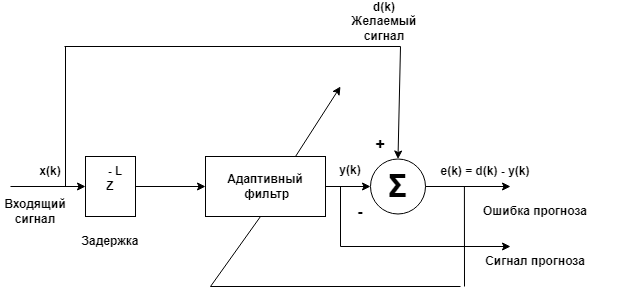
\includegraphics[width=0.9\textwidth]{img/adaptive.png}
  \caption{Блок-диаграмма адаптивного фильтра для предсказания сигналов}
  \label{fig:adaptive}
\end{figure}

\par Не углубляясь в дальнейшие детали реализации необходимо оценить эффективность данного алгоритма в качестве инструмента для предсказания цен акций на реальных биржах. По заявлениям авторов наиболее оптимальным окном предсказания является 15-20 дней, а средняя прибыль составляет около 7\% от объёма инвестиций. Проблематика состоит в том, что статистика для других торговых дней не приведена с формулировкой, что результаты были схожи. Вывод исследования вызывает подозрения о манипулирование путем сокрытия части информации —-- в статье явно не хватает примеров, где фильтр ошибся, и соотношение ошибок и успехов на длительном периоде.
\newpage

\subsubsection{Генетический алгоритм}



\par Генетческий алгортм --— это эвристический алгоритм поиска, используемый для решения задач оптимизации и моделирования путём случайного подбора, комбинирования и вариации искомых параметров с использованием механизмов, аналогичных естественному отбору в природе. Одним из наиболее важных преимуществ генетических алгоритмов является отсутствие необходимости информации о поведении функции и незначительное влияние возможных разрывов на процессы оптимизации. Также как и в случае нейронных сетей, происходит уход от необходимости анализа причинно-следственных связей, путем построения «итогового» образа — целевой функции.

\par Основное преимущество концепции генетического алгоритма —-- это скрещивание, также именуемое комбинированием. В общих чертах идея генетического алгоритма в рамках поставленной задачи сводится к перебору и отбору оптимальной комбинации. Алгоритм делится на следующие этапы:

\begin{itemize}[leftmargin=1.6\parindent]
	\item[---] Скрещивание;
	\item[---] Селекция (отбор);
	\item[---] Формирования нового поколения.
\end{itemize}

\par Вышеперечисленные этапы повторяются до тех пор, пока не будет получен удовлетворительный результат или произойдет одно из ниже перечисленных условий:

\begin{itemize}[leftmargin=1.6\parindent]
	\item[---] Количество поколений достигнет заранее выбранного максимума;
	\item[---] Исчерпано время на мутацию.
\end{itemize}

\par Собственно говоря отсюда и вытекает основной недостаток --- необходимая комбинация для приемлемого результата требует огромных вычислительных мощностей, причём присутствует большая вероятность ее ненахождения. С очень сильной натяжкой целевую функцию можно сравнить со слоем входных нейронов и с ожиданием максимума как аналога максимизации сигнала нейрона выходного слоя. Хотя правильнее было бы говорить, что генетические алгоритмы используются для повышения эффективности обучения нейронных сетей, но все же не могут рассматриваться как конкуренция нейронными сетям.


\subsubsection{Выводы на основе анализа существующих решений}

\par На основе рассмотренных методов можно сделать заключение, о том, что наиболее оптимальным и подходящим решением задачи прогнозирования временных рядов на фондовом рынке является использование нейронных сетей, в сочетание с дополнительными алгоритмами, призванными улучшить их конечную точность. Среди возможных кандидатов наилучшими являются следующие:

\begin{itemize}[leftmargin=1.6\parindent]
    \item[---] Математические модели для анализа прогнозирования стационарных временных рядов;
	\item[---] Генетические алгоритмы для повышения эффективности обучения нейронных сетей;
	\item[---] Сочетание нескольких различных разновидностей архитектуры нейронных сетей.
\end{itemize}

\par В рамках данной работы для разработки кобминированнового метода будут зайдествованы все вышеперечисленные варианты, за исключением генетических алгоритмов, так как на основе предварительного анализа нельзя однозначного утверждать, что они позволяют добиться улучшения прогностической эффективности метода.\cite{genetic, genetic-2}
\pagebreak